%!TEX TS-program = xetex
\documentclass{TDP003mall}
\usepackage[utf8]{inputenc}
\usepackage[swedish]{babel}
%For displaying JSON code in Latex
\usepackage{listings}
\usepackage{xcolor}

\colorlet{punct}{red!60!black}
\definecolor{background}{HTML}{EEEEEE}
\definecolor{delim}{RGB}{20,105,176}
\colorlet{numb}{magenta!60!black}

\lstdefinelanguage{json}{
    basicstyle=\normalfont\ttfamily,
    numbers=left,
    numberstyle=\scriptsize,
    stepnumber=1,
    numbersep=8pt,
    showstringspaces=false,
    breaklines=true,
    frame=lines,
    backgroundcolor=\color{background},
    literate=
     *{0}{{{\color{numb}0}}}{1}
      {1}{{{\color{numb}1}}}{1}
      {2}{{{\color{numb}2}}}{1}
      {3}{{{\color{numb}3}}}{1}
      {4}{{{\color{numb}4}}}{1}
      {5}{{{\color{numb}5}}}{1}
      {6}{{{\color{numb}6}}}{1}
      {7}{{{\color{numb}7}}}{1}
      {8}{{{\color{numb}8}}}{1}
      {9}{{{\color{numb}9}}}{1}
      {:}{{{\color{punct}{:}}}}{1}
      {,}{{{\color{punct}{,}}}}{1}
      {\{}{{{\color{delim}{\{}}}}{1}
      {\}}{{{\color{delim}{\}}}}}{1}
      {[}{{{\color{delim}{[}}}}{1}
      {]}{{{\color{delim}{]}}}}{1},
}

\newcommand{\version}{Version 1.0}
\author{Daniel Huber, \url{danhu849@liu.se}\\
  Jens Öhrnell, \url{jenoh242@liu.se}}
\title{Testdokumentation}
\date{2020-10-22}
\rhead{Daniel Huber\\
Jens Öhrnell}


\begin{document}
\projectpage
\tableofcontents
\section{Revisionshistorik}
\begin{table}[!h]
\begin{tabularx}{\linewidth}{|l|X|l|}
\hline
Ver. & Revisionsbeskrivning & Datum \\\hline
1.1 & Testdokumentation Portfolio TDP003 & 221020 \\\hline
1.0 & Mall för Testdokumentation Portfolio TDP003 & 181020 \\\hline
\end{tabularx}
\end{table}

\section{Information om denna mall}
Författare av dokument som baseras på denna mall är införstådda med reglerna för dess användande. Reglerna återfinns i detta stycke. Varje dokument som är en påbyggnation eller använder delar av detta dokument eller någon av dess senare eller tidigare versioner ska inkludera detta stycke.

Individuella påbyggnationer eller omskrivningar av denna mall förutsätts ha indata och resultat specifierade specifikt för det egna portfolioprojektet. Endast upphovsrättsmannen, Daniel Huber (danhu849) och personer listade nedanför får använda denna mall. Dokumentet får ej delas till andra eller tredje part. Förbrytelser skickas till Diciplinnnämnden vid Linköpings Universitet.
\begin{itemize}
\item Jens Öhrnell, jenoh242
\item Michael Lake, micla389
\item Robin Edlund, robed441
\item Jim Teräväinen, jimte145
\item Ahmed Sikh, ahmsi881
\end{itemize}

Detta samarbete har gjorts möjlig efter mejlkonversation med Examinator för Kursen TDP003, Filip Strömbäck Fredagen 16:e Oktober 2020. Frågor rörande överenskommelsens validitet hänvisas till Filip Strömbäck.
\newpage
\section{Valideringsprogram}
För att uppfylla kraven om korrekt JSON, UTF-8 och Jinja2 i projektet har validerare skrivits i python. JSON valideras av JSON\_tester.py, UTF-8 valideras av utf-8\_tester.py och Jinja2 valideras av jinja2\_validator.py . Även ett program som kontrollerar att alla programfiler skrivits på engelska har skrivits. Koden för samtliga program återfinns i projektrepot.  

\section{Testspecifikation}
Nedan följer tester i ordningen x.n där x motsvaras av det övergripande kravstycket i Universitets \texttt{Systemspecifikation} och n representerar testet i ordningen. Kravet testet uppfyller visas därefter.

Indatan presenteras alltid först. Undertill visas det verkliga resultatet av senaste portfolioversionen ibland av en beskrivning, ibland av en bild och ibland av både och.
\subsection{Tester för presentationslagrets krav}
\subsubsection*{Test 1.1 (Krav 1.1)}
\begin{itemize}
\item[]\textbf{Indata} Öppna portfolion första sida (URL: /).
\item[]\textbf{Resultat} Möts av en header med länkar till: Home, Tekniker och Avancerad Sökning. Nedanför finns sidtitel, en stor bild, introduktionstext, sociala media länkar samt footer med författar info och länk till upphovsrättshavaren av bakgrundsbilden.
\end{itemize}
\subsubsection*{Test 1.2 (Krav 1.2)}
\begin{itemize}
\item[]\textbf{Indata} Öppna portfolio projektlista (URL: /list).
\item[]\textbf{Resultat} Dirigeras till /list sidan och möts av sökfältsknappar, sökbar, en sökknapp och två sorteringslistor. Finns också footer med författar info och länk till upphovsrättshavaren av bakgrundsbilden.
\end{itemize}
\subsubsection*{Test 1.3 (Krav 1.2)}
\begin{itemize}
\item[]\textbf{Indata} Sökning i sökfältet. Endast text, exakt inmatning: 'NEJ' på sidan '/list'.
\item[]\textbf{Resultat} Project number 3: NEJ visas som sökresultat.
\end{itemize} 
\subsubsection*{Test 1.4 (Krav 1.2)}
\begin{itemize}
\item[]\textbf{Indata} Sökning i sökfältet. Endast text, exakt inmatning: 'python' på sidan '/list'.
\item[]\textbf{Resultat} Project number 1, 2 och 3 visas som sökresultat.
\end{itemize}
\subsubsection*{Test 1.5 (Krav 1.2)}
\begin{itemize}
\item[]\textbf{Indata} Klicka på 'ascending' och sedan 'Search' på sidan '/list'.
\item[]\textbf{Resultat} 4 projekt visas med stigande datum från vänster till höger.
\end{itemize}
\subsubsection*{Test 1.6 (Krav 1.2)}
\begin{itemize}
\item[]\textbf{Indata} Ändrar sorteringen från 'fallande' till 'stigande' efter sökning på '/list' med fler än ett resultat. Sorteras på datum. Sedan trycks enter.
\item[]\textbf{Resultat} 4 projekt visas med stigande datum från höger till vänster.
\end{itemize}
\subsubsection*{Test 1.7 (Krav 1.2)}
\begin{itemize}
\item[]\textbf{Indata}Först söks det efter python i sökfältet techniques\_used på /list. techniques\_used i URL:en ändras sedan till enstorkorv. Enter trycks.
\item[]\textbf{Resultat} Det står: Searching for python in search fields: enstorkorv, generated no results.
\end{itemize}
\subsubsection*{Test 1.8 (Krav 1.2)}
\begin{itemize}
\item[]\textbf{Indata} Markerar alla searchfields genom att klicka på dem. Skriver sedan 'e' i sökfältet och trycker sedan enter.
\item[]\textbf{Resultat} Alla projekt visas i sökresultaten.
\end{itemize}
\subsubsection*{Test 1.9 (Krav 1.2)}
\begin{itemize}
\item[]\textbf{Indata}python samt ada markeras på /techniques och sedan klickas det på 'Sök'-knappen.
\item[]\textbf{Resultat} Projekt nummer 2 visas i sökresultaten.
\end{itemize}
\subsubsection*{Test 1.10 (Krav 1.3)}
\begin{itemize}
\item[]\textbf{Indata} Klicka på ett projekt 1 i listan på sidan '/list'
\item[]\textbf{Resultat} Projektsidan för projekt 1 visas.
\end{itemize}
\subsubsection*{Test 1.11 (Krav 1.3)}
\begin{itemize}
\item[]\textbf{Indata} Ändrar URL på projektsidan från 'project/id=3' till 'project/id=4'.
\item[]\textbf{Resultat} Omdirigeras till 404 sida med texten ERROR 404 The page you are trying to reach does not exist.
\end{itemize}
\subsubsection*{Test 1.12 (Krav 1.3)}
\begin{itemize}
\item[]\textbf{Indata} Ändrar URL på projektsidan från 'project/3' till 'project/4'.
\item[]\textbf{Resultat} Projektsidan byts om från projektsidan för projekt 3 till projektsidan för projekt 4.
\end{itemize}
\subsubsection*{Test 1.13 (Krav 1.4)}
\begin{itemize}
\item[]\textbf{Indata} Alla tekniker på '/techniques' sidan markeras. Sedan trycks enter.
\item[]\textbf{Resultat} Inga projekt visas.
\end{itemize}
\subsubsection*{Test 1.14 (Krav 1.5)}
\begin{itemize}
\item[]\textbf{Indata} Kontrollera att ett sökresultat på sidan /list har små bilder genom att inspektera element. 
\item[]\textbf{Resultat} Inspektion av element ger:\\ \texttt{<img src="https://via.placeholder.com/300" alt="XXX" style="float: left;">} Bilden är 150px stor.
\end{itemize}
\subsubsection*{Test 1.15 (Krav 1.5)}
\begin{itemize}
\item[]\textbf{Indata} Kontrollera att projektsidan '/project/1/' har minst en stor bild genom att inspektera element på sidan.
\item[]\textbf{Resultat} Inspektion av element ger:\\ \texttt{<img src=''https://via.placeholder.com/300'' alt=''XXX'' style=''float: left;''\\ data-module='''' test='''' script=''''>} Bilden är 300px stor.
\end{itemize}
\subsubsection*{Test 1.16 (Krav 1.6)}
\begin{itemize}
\item[]\textbf{Indata} Efter sökning med search\_field small\_image i '/list'. Sätt 'search\_field' variabeln i URL:en till 'lKAsm32105,saölf'.
\item[]\textbf{Resultat} Följande text visas: Searching for in search fields: lKAsm32105,saölf, generated no results.
\end{itemize}
\subsubsection*{Test 1.17 (Krav 1.7)}
\begin{itemize}
\item[]\textbf{Indata} Ändra URL:en på projektsidan \texttt{'project/3' till 'project/a'}
\item[]\textbf{Resultat} Sidan omdirigeras till en sida med texten ERROR 404 The page your are trying to reach does not exist.
\end{itemize}
\subsubsection*{Test 1.18 (Krav 1.7)}
\begin{itemize}
\item[]\textbf{Indata} Ändra URL:en på projektsidan 'project/3' till 'project/854965625'.
\item[]\textbf{Resultat} Sidan omdirigeras till en sida med texten ERROR 404 Project with project id: 854965625 does not exist. 
\end{itemize}




\subsection{Tester för datalagrets krav}
\subsubsection*{Test 2.1 (Krav 2.1, 2.2, 2.3, 2.4)}
\begin{itemize}
\item[]\textbf{Indata} Ändra import datalager as data till import daniel\_data as data i filen data\_test.py. Skriv \texttt{./data\_test.py} i terminalen.
\item[]\textbf{Resultat:}
\begin{figure}[h!]
\centerline{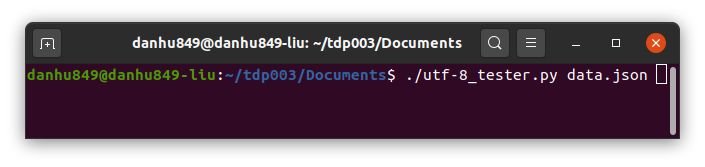
\includegraphics[width=\textwidth, height=4cm]{../Pictures/utf-8_tester_test.png}}
\caption{Resultatet av data\_test.py körning.\label{fig:1}}
\end{figure}
\end{itemize}
\newpage
\subsubsection*{Test 2.2 (Krav 2.7)}
\begin{itemize}
\item[]\textbf{Indata:}
\begin{figure}[h!]
\centerline{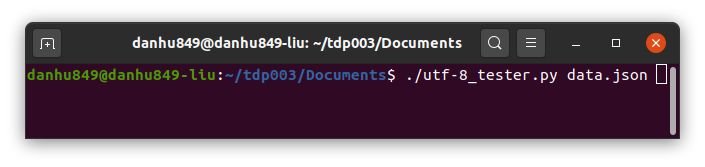
\includegraphics[width=\textwidth, height=3.5cm]{../Pictures/utf-8_tester_test.png}}
\caption{Hur programmet utf-8\_tester.py körs i terminalen.\label{fig:2}}
\end{figure}
\item[]\textbf{Resultat:}
\begin{figure}[h!]
\centerline{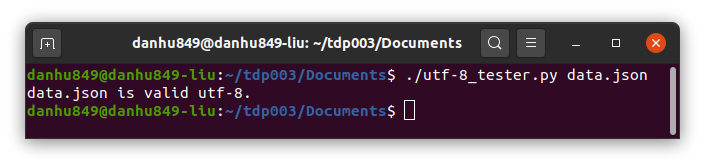
\includegraphics[width=\textwidth, height=3.5cm]{../Pictures/utf-8_tester_valid.png}}
\caption{Resultat från att köra utf-8\_tester.py\label{fig:3}}
\end{figure}
\end{itemize}
\subsubsection*{Test 2.3 (Krav 2.8)}
\begin{itemize}%Lägga till data.json i Appendix A
\item[]\textbf{Indata} Lägg till ett projekt med ett till sökfält, 'new\_search\_field' i data.json. Se Appendix B. Testa sedan att köra hemsidan med flask run. Sök på 'new' med sökfältet 'new\_search\_list' markerat i /list.
\item[]\textbf{Resultat} Bara det nyligen tillagda projektet ges som sökresultat.
\end{itemize}
\subsubsection*{Test 2.4 (Krav 2.9)}
\begin{itemize}
\item[]\textbf{Indata} flask session startas utan debug\_mode och ett femte projekt läggs till manuellt i data.json medan flask kör. Sedan öppnas /list i webläsaren.
\item[]\textbf{Resultat} Alla fem projekt laddas in.
\end{itemize}


\newpage
\subsection{Tester för Icke-funktionella Krav}
\subsubsection*{Test 3.1 (Krav 3.1)}
\begin{itemize}
\item[]\textbf{Indata} Validera Jinja2 i samtliga HTML filer i '/templates' genom att köra Jinja2 valideraren: jinja2\_validator.py med /templates mappen som argument i terminalen.
\item[]\textbf{Resultat:}
\begin{figure}[h!]
\centerline{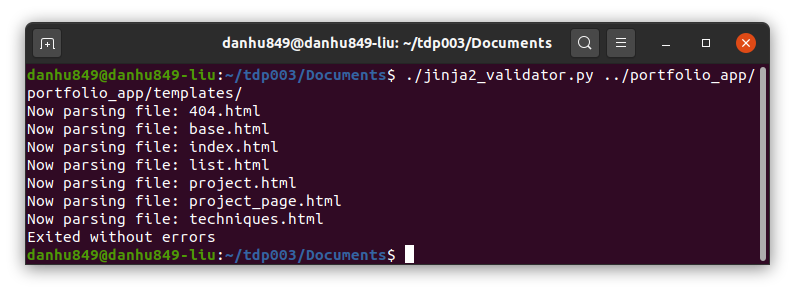
\includegraphics[width=\textwidth, height=5cm]{../Pictures/jinja2_validated.png}}
\caption{Resultat från att köra jinja2\_validator.py\label{fig:4}}
\end{figure}
\end{itemize}
\subsubsection*{Test 3.3 (Krav 3.2)}
\begin{itemize}
\item[]\textbf{Indata} Validera portfoliosidans css3 med hjälp av w3 css3 validerare:\\ \texttt{https://jigsaw.w3.org/css-validator/}\\Sätt 'Profile: CSS level 3', 'Medium: All', 'Warnings: Normal report', 'Vendor Extensions: Default'.
\item[]\textbf{Resultat:}
\begin{figure}[h!]
\centerline{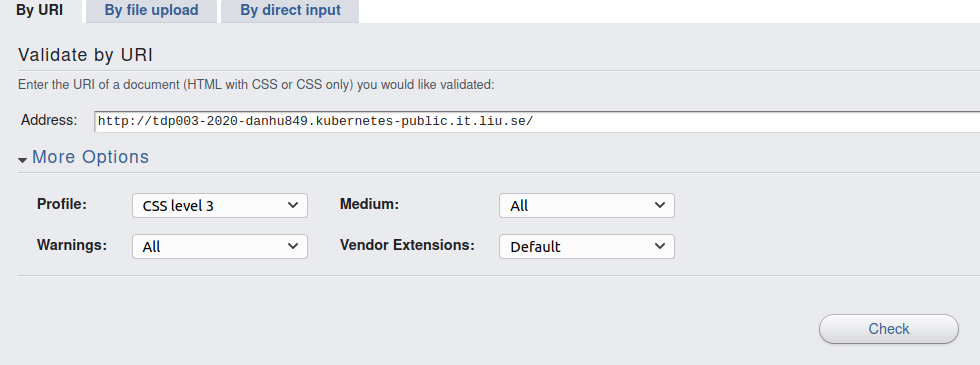
\includegraphics[width=\textwidth, height=5cm]{../Pictures/css3_validation.png}}
\caption{Resultat från att köra w3:s css3 validerare.\label{fig:5}}
\end{figure}
\end{itemize}
\newpage
\subsubsection*{Test 3.4 (Krav 3.2)}
\begin{itemize}
\item[]\textbf{Indata} Validera portfoliosidans HTML5 med hjälp av w3:s HTML5 validerare:\\\texttt{https://validator.w3.org/\#validate\_by\_uri+with\_options}
  \begin{figure}[h!]
\centerline{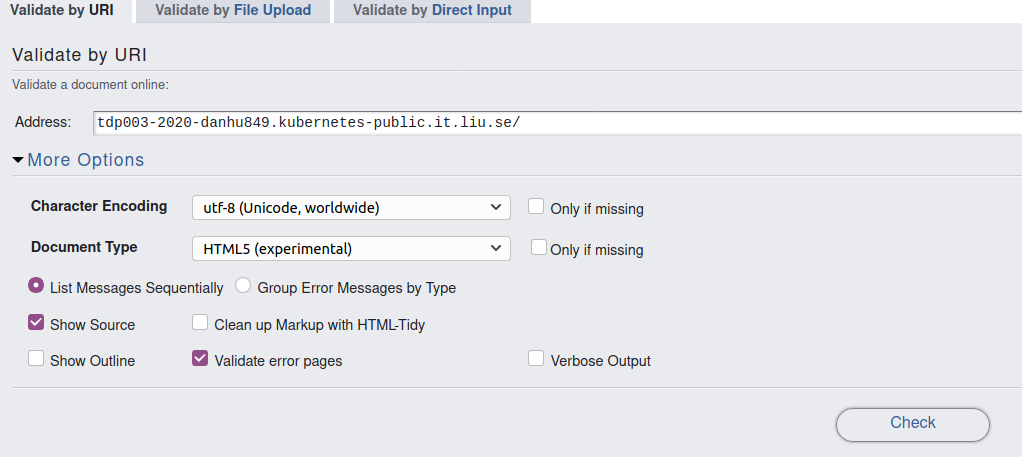
\includegraphics[width=\textwidth, height=5cm]{../Pictures/HTML5_check.png}}
\caption{Inställningar för w3 HTML5 validering.\label{fig:6}}
\end{figure}
\item[]\textbf{Resultat:}
    \begin{figure}[h!]
\centerline{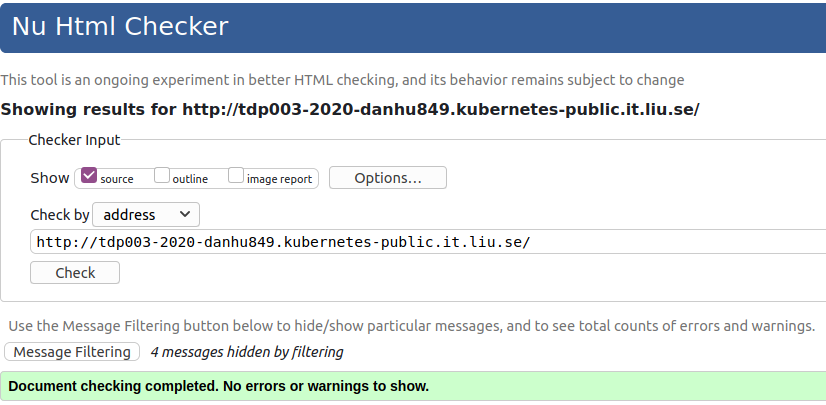
\includegraphics[width=\textwidth, height=5cm]{../Pictures/HTML5_check_result.png}}
\caption{Resultat av w3 HTML5 validering.\label{fig:7}}
\end{figure}
\end{itemize}
\newpage
\subsubsection*{Test 3.5 (Krav 3.3)}
\begin{itemize}
\item[]\textbf{Indata} I terminalen: cd till projektets katalog. Skriv ut katalogens innehåll med tree kommandot som syns på resultatbilden \ref{fig:8}. 
\item[]\textbf{Resultat:}
  \begin{figure}[h!]
\centerline{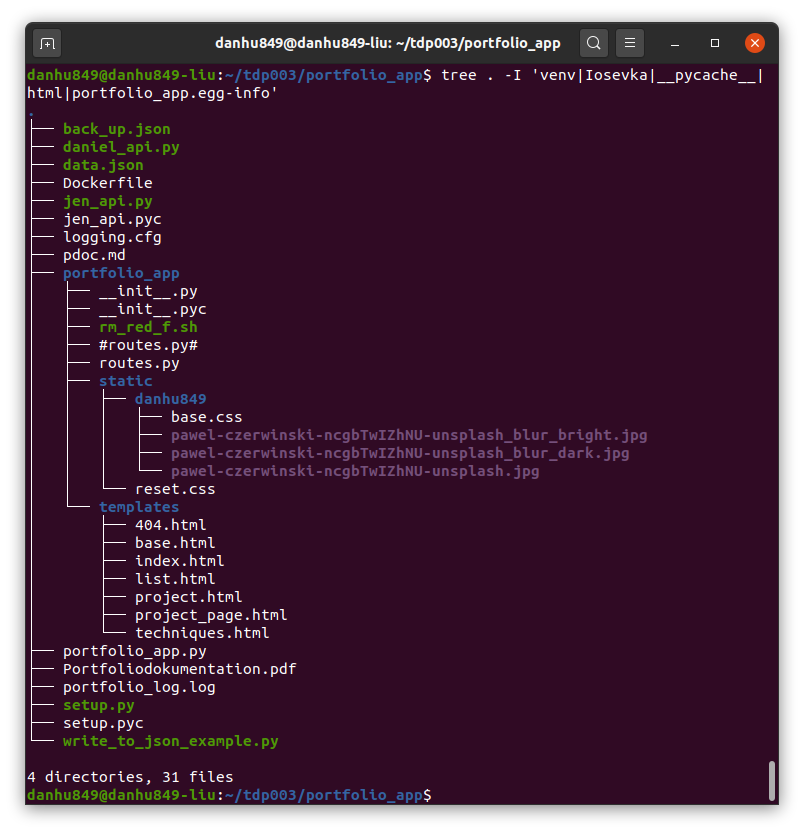
\includegraphics[width=\textwidth, height=12cm]{../Pictures/app_tree.png}}
\caption{Resultat från att trädkommandot tree i terminalen.\label{fig:8}}
\end{figure}
\end{itemize}
\newpage
\subsubsection*{Test 3.6 (Krav 3.4)}
\begin{itemize}
\item[]\textbf{Indata} Bevisa att projektet versionhanteras med git genom att visa print screen över repots 'Value Stream Analytics'.
\item[]\textbf{Resultat:}
\begin{figure}[h!]
\centerline{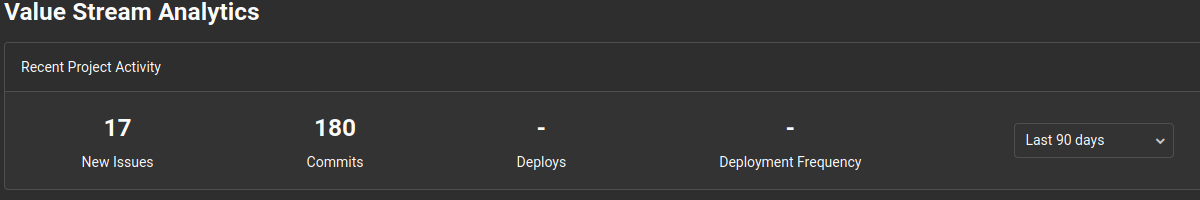
\includegraphics[width=\textwidth, height=3cm]{../Pictures/value_stream.png}}
\caption{Print Screen över Value Stream Analytics portfolio repots Analytics tab.\label{fig:9}}
\end{figure}
\end{itemize}

\subsubsection*{Test 3.7 (Krav 3.5)}
\begin{itemize}
\item[]\textbf{Indata} Bevisa att presentationen av systemet är godkänd och lägg till kommentarer från användare från klassens portfolio presentation.
\item[]\textbf{Resultat} %Inscanning av det dokumentet i appendix 
\end{itemize}
\subsubsection*{Test 3.8 (Krav 3.6, 3.7)}
\begin{itemize}
\item[]\textbf{Indata} cd till \texttt{/tdp003/Documents}. chmod check\_if\_english.py om det behövs för att göra \\check\_if\_english.py exekverbar. Kör programmet i terminalen: \texttt{./check\_if\_eng.py wordlist\_eng.txt ../portfolio\_app/} Skriv ut innehållet för alla filer med \texttt{cat uword\_directory/*} och kontrollera att de okända orden endast är programmeringstermer.
\item[]\textbf{Resultat} 
\end{itemize}
\subsubsection*{Test 3.9 (Krav 3.8, 3.9 och 3.10)}
\begin{itemize}
\item[] Se dokumentet \texttt{danhu849\_jenoh242\_Systemdokumentation.pdf} i portfolions repo:\\
  \texttt{https://gitlab.liu.se/jenoh242/tdp003/-/tree/master/Documents}
\end{itemize}





\section{Testlogg}

\begin{tabular}{|l|l|l|l|l|}
  \hline
  Datum & Commit & Godkända & Avvikande & Kommentar \\ [0.5ex]
  \hline
  2019-10-22 & bfc02812 & Alla & - & - \\
  \hline
  \hline
  2019-10-21 & 13926161 & - & 1.7, 1.8, 1.16 &10 projekt kommer upp istället för de förväntade 4.\\
  \hline
  \hline
\end{tabular}

\newpage
\appendix
\section{Data.json}
\lstinputlisting[language=JSON]{data.json}
\section{Feedback - Presentation av Portfolio}


\end{document}
%Formateringsexempel

%% \begin{itemize}
%%     \item 
%%     \item 
%%     \item 
%%     \item 
%%     \item 
%%     \item 
%% \end{itemize}

%% \begin{figure}[h]
%%   \centerline{
\includegraphics[width=\textwidth, height=10cm]{ida.png}}
%%   \caption{ \label{fig:2}}
%% \end{figure}

%% \ref{fig:2} 



%%% Local Variables: 
%%% coding: utf-8
%%% mode: latex
%%% TeX-engine: xetex
%%% TeX-master: t
%%% End: 
